\documentclass[11pt]{article}
\usepackage{setspace}
\setstretch{1}
\usepackage{amsmath,amssymb, amsthm}
\usepackage{graphicx}
\usepackage{bm}
\usepackage[hang, flushmargin]{footmisc}
\usepackage[colorlinks=true]{hyperref}
\usepackage[nameinlink]{cleveref}
\usepackage{footnotebackref}
\usepackage{url}
\usepackage{listings}
\usepackage[most]{tcolorbox}
\usepackage{inconsolata}
\usepackage[papersize={8.5in,11in}, margin=1in]{geometry}
\usepackage{float}
\usepackage{caption}
\usepackage{esint}
\usepackage{url}
\usepackage{enumitem}
\usepackage{subfig}
\usepackage{wasysym}
\newcommand{\ilc}{\texttt}
\usepackage{etoolbox}
\usepackage{algorithm}
\usepackage{changepage}
% \usepackage{algorithmic}
\usepackage[noend]{algpseudocode}
\usepackage{tikz}
\usetikzlibrary{matrix,positioning,arrows.meta,arrows}
\patchcmd{\thebibliography}{\section*{\refname}}{}{}{}
% \PassOptionsToPackage{hyphens}{url}\usepackage{hyperref}

\providecommand{\myceil}[1]{\left \lceil #1 \right \rceil }
\providecommand{\myfloor}[1]{\left \lfloor #1 \right \rfloor }


\begin{document}



\title{\textbf{CSDS 455: Homework 13}}

\author{Shaochen (Henry) ZHONG, \ilc{sxz517}}
\date{Due and submitted on 10/07/2020 \\ Fall 2020, Dr. Connamacher}
\maketitle


\section*{Problem 1}

We will have the following diagram for a base graph:

\begin{figure}[H]
    \centering
    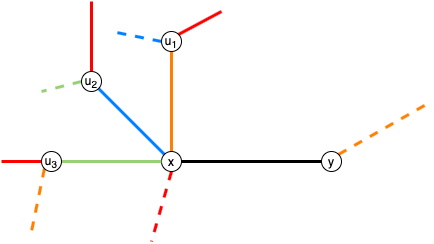
\includegraphics[width=0.6\linewidth]{{fig/fig_p1_1.png}}
    \caption{Base graph for \textit{Problem 1}}
    \label{fig:p1_1}
\end{figure}

For better clarity, we have $u_1, u_2, ..., u_i \in N(x)$ being the adjacent vertices of $x$ excluding $y$. Known that $\chi'(G-xy) = \Delta + 1$, every vertex in $G-xy$ must be missing\footnote{``Missing'' in this context means not having a edge of a certain color. ``Vertex $v$ is missing color $c$'' means there is no edge of color $c$ connected to $v$} at least one color from the $\Delta +1$ colors, we use dashed lines to represent such colors. We also use solid lines to represent the color of edges under a $\Delta + 1$ edge-coloring of $G-xy$. We will also use some arbitary actual color names to help understanding.\newline

\noindent We want to show that other than having an 2-color alternating path between $x$ and $y$, we will always have $\chi'(G) = \Delta + 1$, thus a contradiction.\newline

\subsection*{Proposition 1. $x$ and $y$ can't miss the same color.}

This observation is almost trivial as otherwise we may just color edge $xy$ with this color, then we have a $\Delta + 1$ coloring of $G$ -- a contradiction.

\subsection*{Proposition 2. $x$ must include every missing color of $N(x)$.}
Say we have a set $S$ which include all the missing colors of $N(x)$, such $S$ must be a subset of the colors connected $x$. This is because if we have a vertex $u_i \in N(x)$ which has a missing color of \textcolor{purple}{purple} which is not included in the connected colors of $x$, we have two cases.

First, $u_i$ is $u_1$, where edge $u_1x$ has the color which $y$ misses, then we may recolor the graph as following. Which will make $x$ and $y$ both missing \textcolor{orange}{orange}; we can therefore color $xy$ with \textcolor{orange}{orange} and have a $\Delta + 1$ coloring of $G$ -- a contradiction.

\begin{figure}[H]
    \centering
    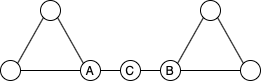
\includegraphics[width=0.8\linewidth]{{fig/fig_p1_2.png}}
\end{figure}



Second, we may have $u_ix$ not having the color which $y$ misses. We can then recolor $u_ix$ to be \textcolor{purple}{purple}, and recolor the original \textcolor{blue}{blue} $u_jx$ ($u_j$ is another neighbor vertex of $x$ which is missing \textcolor{green}{green}) to be \textcolor{green}{green}, and recolor another neighbor vertex of $x$ which is missing the color of $u_jx$... Take $u_3 = u_i$ as an example, we will have:


\begin{figure}[H]
    \centering
    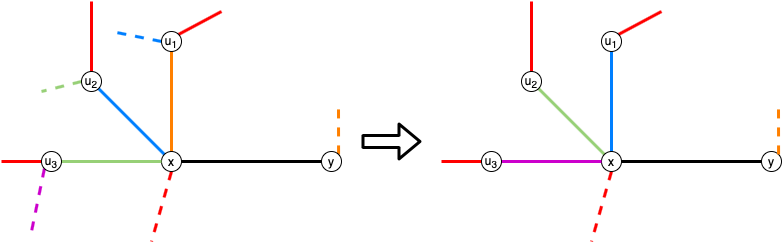
\includegraphics[width=0.8\linewidth]{{fig/fig_p1_3.png}}
\end{figure}

We know this recoloring method works since $N(x)$ is finite, so we will always able to recolor $u_1x$ (\textcolor{orange}{orange}, which $y$ misses) to the missing color of $u_1$ (\textcolor{blue}{blue}), then recolor the \textcolor{blue}{blue} edge $u_jx$ to its missing color, then .... we will eventually reaches $u_i$ and recolor $u_ix$ to its missing color \textcolor{purple}{purple}. Then we will have $x$ and $y$ both missing \textcolor{orange}{orange} and thus a contradiction.\newline

Now we have showed that every missing color of $N(X)$ must show on an edge of $ux$ for $u \in N(x)$. Be familiar with this recoloring method as we will use it later.


\subsection*{Proposition 2. If $x$ misses \textcolor{red}{red}. Every $u \in N(x)$ must have an \textcolor{red}{red} edge connected to $u$.}

Because otherwise, by using the recolring method introduced in \textbf{Proposition 2}, we may have $x$ and $y$ both missing \textcolor{orange}{orange} and thus a contradiction. The following is an example assuming $u_3$ missing \textcolor{red}{red}, but it can be any $u \in N(x)$.

\begin{figure}[H]
    \centering
    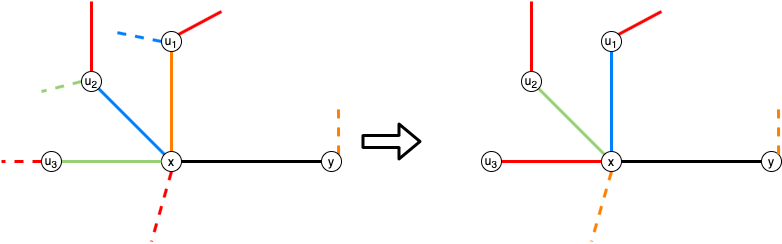
\includegraphics[width=0.8\linewidth]{{fig/fig_p1_4.png}}
\end{figure}

Combining the finding of \textbf{Proposition 1, 2, 3}, we will have a graph like [Figure \ref{fig:p1_1}].






\section*{Problem 2}

% \section{References}
%
% \nocite{*}
% \raggedright
% \bibliography{references.bib}
% \bibliographystyle{plain}


\end{document}